\chapter{Modelo de integración de la información}

Las nuevas tecnologías de análisis genético son fáciles y económicas de hacer lo que genera una gran cantidad de datos biológicos y lo que hace que los biólogos trabajen cada vez más con las nuevas tecnologías de análisis genético, haciendo que los biólogos trabajen más y más computacionalmente.Especialmente mediante el uso de  tecnologías de secuenciación (NGS) y presentar un reto para integrar y almacenar la información, pasos que son necesarios para su posterior análisis \cite{Li2014,Cook2016}.\\

La gran cantidad de datos presentan un reto para organizar y manejar datos que crecen de manera exponencial y que son de diversos tipos, dado que los datos son generados a diferentes niveles y con diferentes métodos (ejemplo: Variantes de exones o imágenes de patología), datos que a su vez deben ser almacenados en distintas formas, esta situación muestra una seria dificultad para realizar un análisis integral de los datos \cite{Cook2016,Li2014}.\\

El mayor de los retos es crear herramientas que permitan al investigador acceder a la información fácilmente y que pueda tener una base de datos intercalable,donde pueda consultar, analizar y actualizar la información de sus experimentos \cite{Li2014}.En el campo clínico esto representa un reto aun mayor dado que se hace necesario recolectar los datos genéticos junto con los datos clínicos para poder hacer análisis más acertados y a gran escala \cite{Paila2013}.\\

El problema de la heterogeneidad  de los datos  se aplica igualmente a los datos clínicos que describen pacientes individuales y además a los datos biológicos que caracterizan nuestro genoma. Específicamente la información genómica y clínica son datos altamente heterogéneos con respecto a los modelos de datos que emplean normalmente, los esquemas de datos que especifican, los lenguajes de consulta que soportan y las terminologías que reconocen \cite{Sujansky2001}.\\

Para el caso de las variantes se tiene que para cada individuo hay 3.5 millones de variantes por individuo, estas variantes son almacenadas normalmente en el formato VCF (Formato de llamado de variantes), a su vez estos archivos pueden contener varias gigas de información,especialmente las muestras de genomas completos, que representan un problema para el almacenamiento dentro de las bases de datos, bases de datos que han sido desarrolladas para dar soluciones dependientes de las diferentes características y necesidades de los laboratorios\cite{Kutzera2017}.\\

Por ello se hace necesario que se utilicen herramientas para la gestión de la información, por ejemplo django que es un web framework de alto nivel desarrollado en python  fomenta el desarrollo rápido y limpio, para la creación de aplicaciones web, es de código abierto y gratuito.Se basa en los principios de desarrollo rápido, manejo de la seguridad y es altamente escalable . Dentro de las muchas aplicaciones que tiene django una es el manejo y gestión de bases de datos a través de los módulos de python. https://www.djangoproject.com/. 

Este capítulo esta organizado en 1. Diseño e implementación de datos. 2. Gestión de datos clínicos y genómicos. 3. Conclusiones. 4. Resumen.

\section{Diseño e implementación del modelo de datos}

A continuación proponemos la utilización de una base de datos con información clínica  y las variantes obtenidas a partir del pipeline. La figura \ref{fig:flujo2} representa el esquema de datos que fue utilizado para realizar la integración de la información dentro de la base de datos.

\begin{figure}[H] 
	\centering
	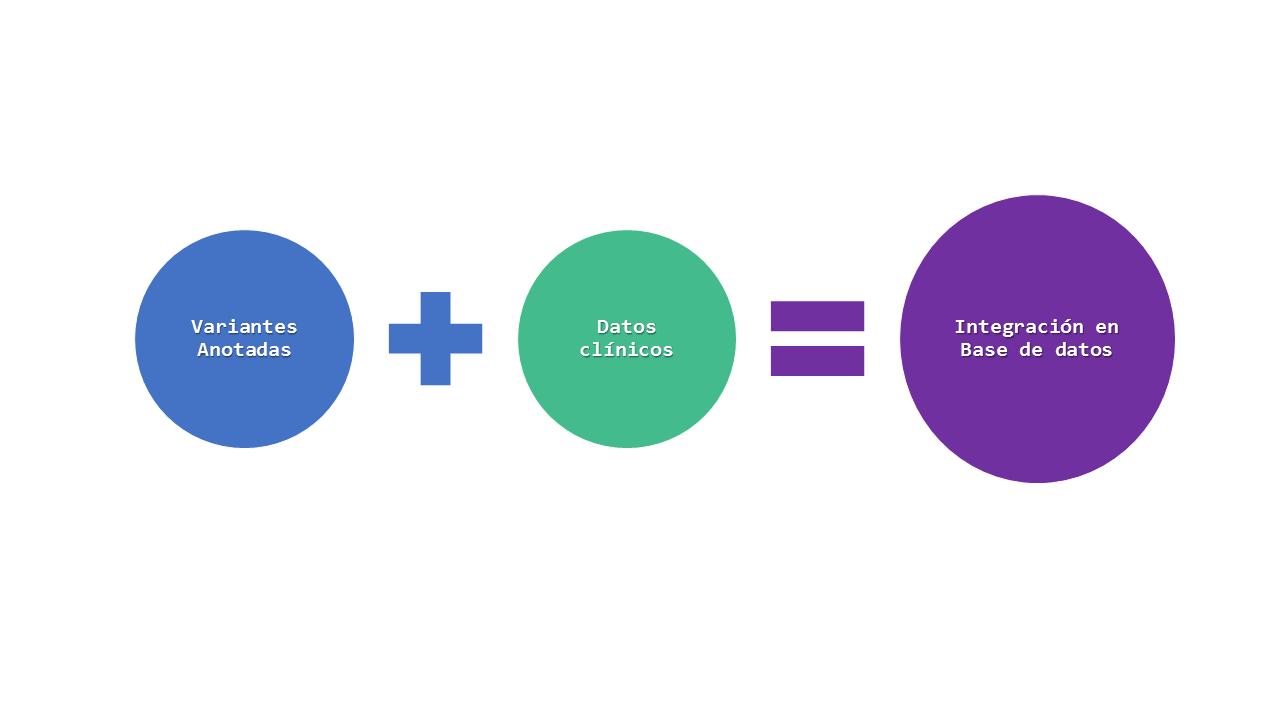
\includegraphics[width=0.5\textwidth]{Kap3/flujo2}
	\caption{Esquema de datos integrados} 
	\label{fig:flujo2}
\end{figure}

Teniendo en cuenta la información a utilizar se diseño el esquema EER  que muestra la figura \ref{fig:t} con las tablas generadas por la aplicación para crear la base de datos propias de Django y las tablas de para la gestión del las variantes junto con la historia clínica.

\begin{figure}[H]
	\centering
	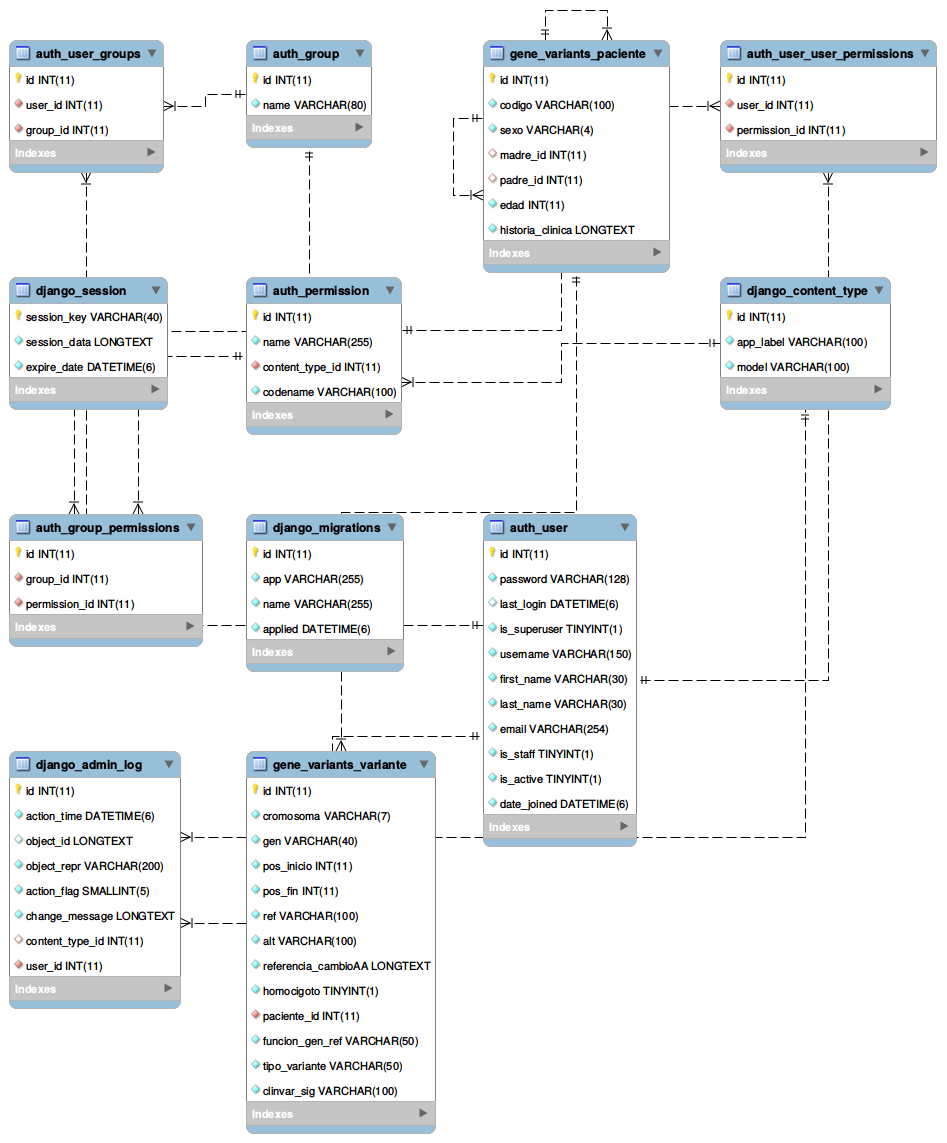
\includegraphics[width=0.9\textwidth]{Kap3/modeloEER}
	\caption{Modelo entidad relación} \label{fig:t}
\end{figure}

Las tablas diseñadas para gestionar las variantes y las historias clínicas son gene\_variants\_paciente que contienen:

\begin{itemize}
	\item Edad: 0-99. Los recién nacidos  o menores de un año tienen una edad de 0.
	\item Sexo: F o M según corresponda.
	\item Descripción: Que corresponde a la información clínica disponible.
\end{itemize} 

Las historias clínicas fueron transcritas manualmente y cargadas desde un archivo de texto plano con un formato especifico.\\

Las variantes con su historia clínica fueron cargadas mediante un script en bash disponible en https://github.com/jevelezse/variantesBD/blob/master/carga.bash, donde se toman los archivos .csv de annovar junto con los archivos de texto que tienen la información clínica del paciente distribuida de la siguiente forma:

\section{Gestión de datos genómicos y clínicos}

Los resultados obtenidos fueron una aplicación con una interfaz que permite a los usuarios con poco conocimiento de  programación  analizar los datos de variantes y su resumen de la historia clínica. \\

\begin{figure}[h] 
	\centering
	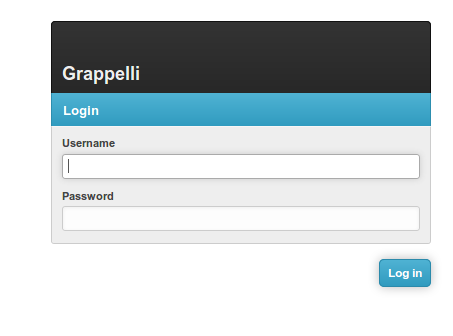
\includegraphics[width=0.4\textwidth]{Kap3/admin_django}
	\caption{Interfaz de ingreso para  administrar la base de datos.} \label{fig:admin}
\end{figure}

Inicialmente la figura\ref{fig:admin}, muestra la solicitud de usuario y contraseña para acceder a la aplicación, es diferente a la base de MySQL, pero  puede tener  una contraseña igual o diferente a la de la base de datos.

\begin{figure}[h] 
	\centering
	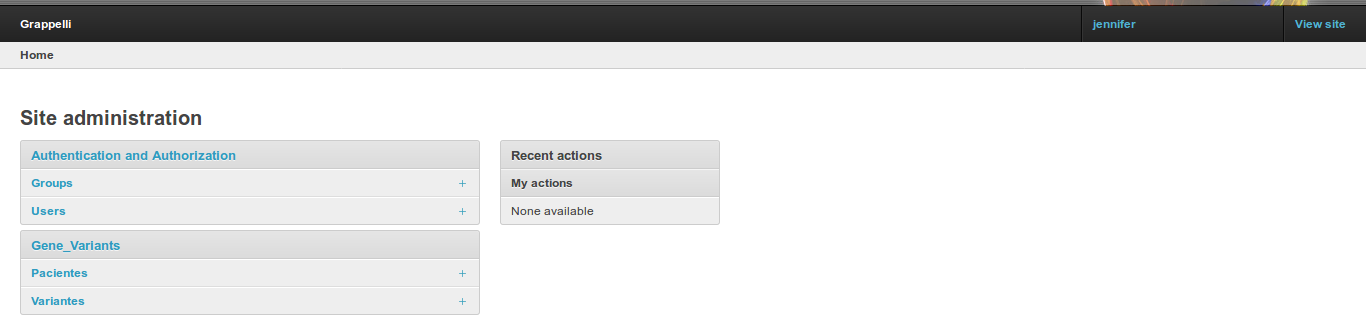
\includegraphics[width=0.5\textwidth]{Kap3/django_admin}
	\caption{Interfaz de administración.} \label{fig:admin2}
\end{figure}

La figura \ref{fig:admin2}, muestra el sitio de administración donde se encuentran los usuarios permitidos, las bases de datos a consultar y muestra un histórico de las actividades recientes. \\

Desde esta interfaz se puede agregar un grupo, más usuarios, pacientes y/o variantes dando click en el signo más sin necesidad de hacer la carga directa a MySQL ya que Django se encarga de hacer la carga, lo que permite actualizar los cambios que se reporten para la variante, por ejemplo variantes que por su alta frecuencia poblacional dejan de ser variantes y se convierten en referencias. \\

\begin{figure}[h] 
	\centering
	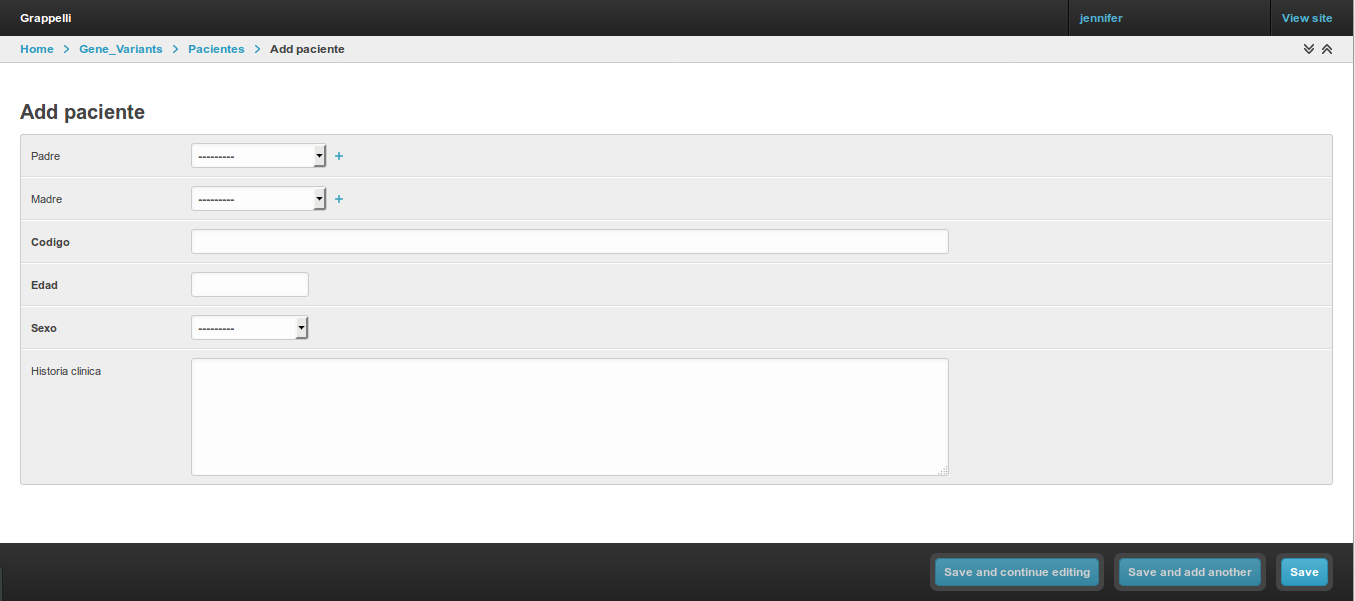
\includegraphics[width=0.5\textwidth]{Kap3/ingresar_paciente}
	\caption{Ingreso de pacientes.} \label{fig:pacientes}
\end{figure}

En la figura \ref{fig:pacientes} se muestra el formulario para ingresar una nueva historia o de modificar una historia clínica de un paciente de manera manual.

\begin{figure}[h] 
	\centering
	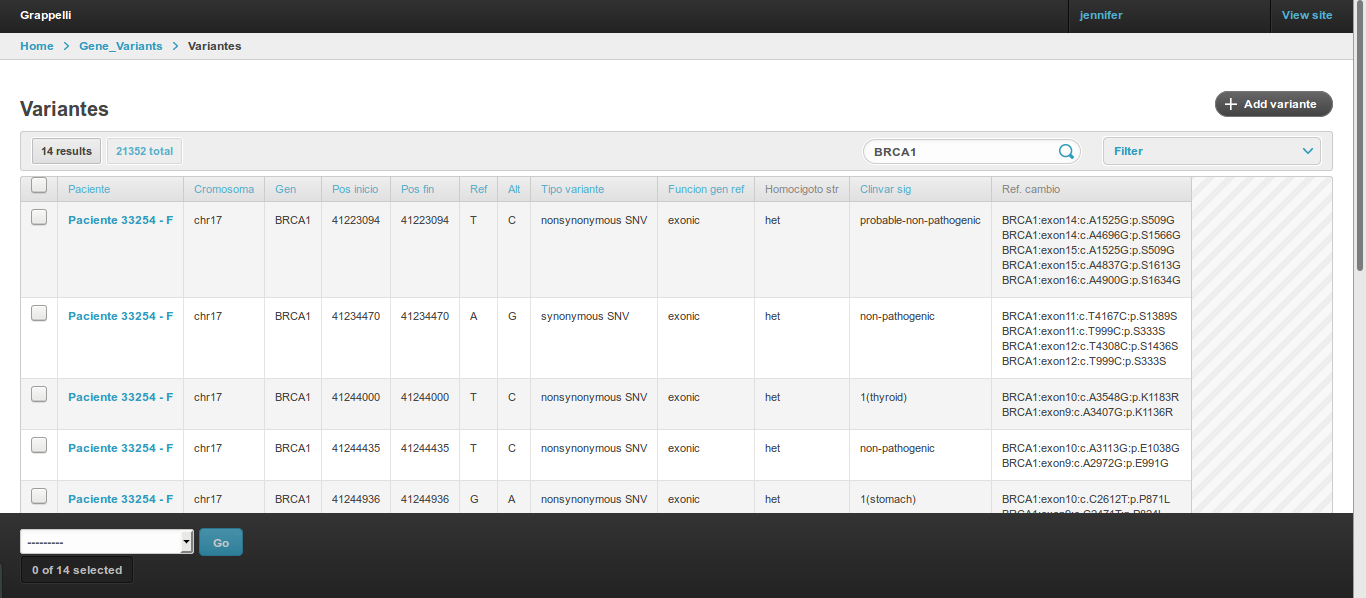
\includegraphics[width=0.5\textwidth]{Kap3/consulta}
	\caption{Consulta a variantes} \label{fig:consulta}
\end{figure}


La figura \ref{fig:consulta} muestra una consulta de las variantes que se tienen cargadas en la base de datos para el gen BRCA1, donde nos muestra una consulta de las variantes con su anotación  filtrada mediante un script de python antes de cargar las anotaciones de la tabla obtenida por annovar para cada paciente. Desde esta misma interfaz se puede hacer consultas de pacientes que se deben eliminar, en la parte inferior se encuentra la opción.\\

Si se desea hacer modificaciones a los datos del paciente también es posible hacerlo desde esta misma interfaz seleccionando el código del paciente, que lleva a la tabla de genes\_varante\_paciente que contiene el formulario de la historia clínica con los datos cargados para ser modificados. 

La importancia de gestión aplicada al manejo de datos clínicos y de información genética es de vital importancia dado que existen miles de anotaciones que requieren de scripts para cargarlos las anotaciones y como es este caso el historial clínico del paciente \cite{Paila2013}. \\

La aplicación desarrollada para crear y gestionar una base de datos aplicada una bioinformática con aplicaciones a la medicina, es necesario que la base de datos provea las consultas para soportar las decisiones sobre un paciente en especifico teniendo en cuenta sus datos,la relación con datos de otros pacientes y los datos de exomas, además de los datos relacionados con los familiares en caso de que se encuentren estos datos. Mostrando que es posible realizar una integración adecuada de los datos bioinformáticos y clínicos utilizando bases de datos relacionales, con una buena respuesta en las consultas. \cite{Sujansky2001}.

\section{Conclusión}

La utilización de aplicaciones en Django permite que un bioinformático diseñe e implementar bases de datos aplicadas al diagnostico clínico, donde se puede guardar y gestionar toda la información obtenida de un paciente, lo que permite hacer análisis a profesionales Médicos y biólogos fácilmente. Una vez ha sido implementa la base de datos también es posible aplicar técnicas de minería de datos para optimizar los análisis de la información. \\

\section*{Resumen}

En este capitulo se presento el proceso de diseñar e implementar un sistema de información para la gestíon de datos clínicos y genómicos, dada la importancia de tener toda la información integrada para hacer futuros análisis. Se utilizo la herramienta de Django como gestor de la base de datos, se transcribió las historias clínicas y se cargaron las variantes obtenidas para cada paciente, como resultado se genero un sistema de información que permite realizar consultas de variantes con las características clínicas de los pacientes.   